\chapter{Analysis}

\section{Introduction}

\subsection{Client Identification} 
My client is Tom Wolf, he is 46 and he is my A level ICT teacher. Tom teaches A level ICT, Doploma ICT and GCSE ICT at Long Road sixth form college. As he is an ICT teacher, he is very educated in computer related subjects, but his programming experience is relatively small and he is not able to write complex programs programs for himself

\subsection{Define the current system} 
Currently the system is Tom himself and Google Drive and/or his hard drive on his laptop used to store calculated data. Tom is required to collect grades of student from the school system, use an algorithm to calculate his/her predicted grade, create a table using already purcheased software such as Microsoft Word and  insert new calculated data to the table. This is very time consuming, as he is required to repeat this process after few assignments.

\subsection{Section appendix}

Summerised Interview

What sort of system do you need currently?
-It has to be an electronic equivalent of a markbook
-It should be able to store infinite amount of units, which represent a term (spring term, autumn term,etc)
-Within the units should be assignments
-Assignments represent exams, school work, tests grades, etc.
-The number of assignments within a unit also shouldn't have limitation
-Predicted grade should be calculated in the program, for an assignment a maximum mark should be assigned and for every student, a mark should be given
-Using a specific algotithm, a grade should be calculated
-Using the grades from the assignments, a predicted grade for the end of the unit and the end of the year should be calculated
-The system should also be capable of calculating the average grade for the whole class for the assignment, unit, and the average predicted grade for the whole class.
-Additionally, it is not required, the system should have a function to calculate the average predicted grade for the whole year
-Calculating the grade for A2 and AS should use a different algorithm

\subsection{Describe the problems}

Tom is required to calculate predicted grades for 200 students by himself and this requires his own time, so the school does not pay him for this. So, for Tom this is not satisfactory as 200 students is a big amount and so it requires a lot of effort and time. Therefore, Tom requires software that will perform those calculations automatically. 

\section{Investigation}

\subsection{The current system}
\subsubsection{Data sources and destinations}

In the current system, after Tom marks his students' course work, assesments, etc., he then has to count up the total marks and write the grade in his markbook or google drive database. Then based on the mark scheme, he sets the grade (either in google drive or his markbook) and the predicted grade for the end of the year. Predicted grade has to be calculated every term, so this is a lot of effort as well (as there are 200 students in total).

\subsubsection{Algorithms}
At this point I am aware of the following algorithms:
-Calculating the end of the unit predicted grade

-Calculating the end of the year predicted grade (for AS)

-Calculating end of the year predicted grade(for A2)

-Calculating the grade

-Calculating average predicted end of the year grade for the whole class

-Calculating average predicted  end of the unit grade for the whole class

-Calculating average end of the year grade for the whole class



\subsubsection{Data flow diagram}

\begin{figure}[H]
    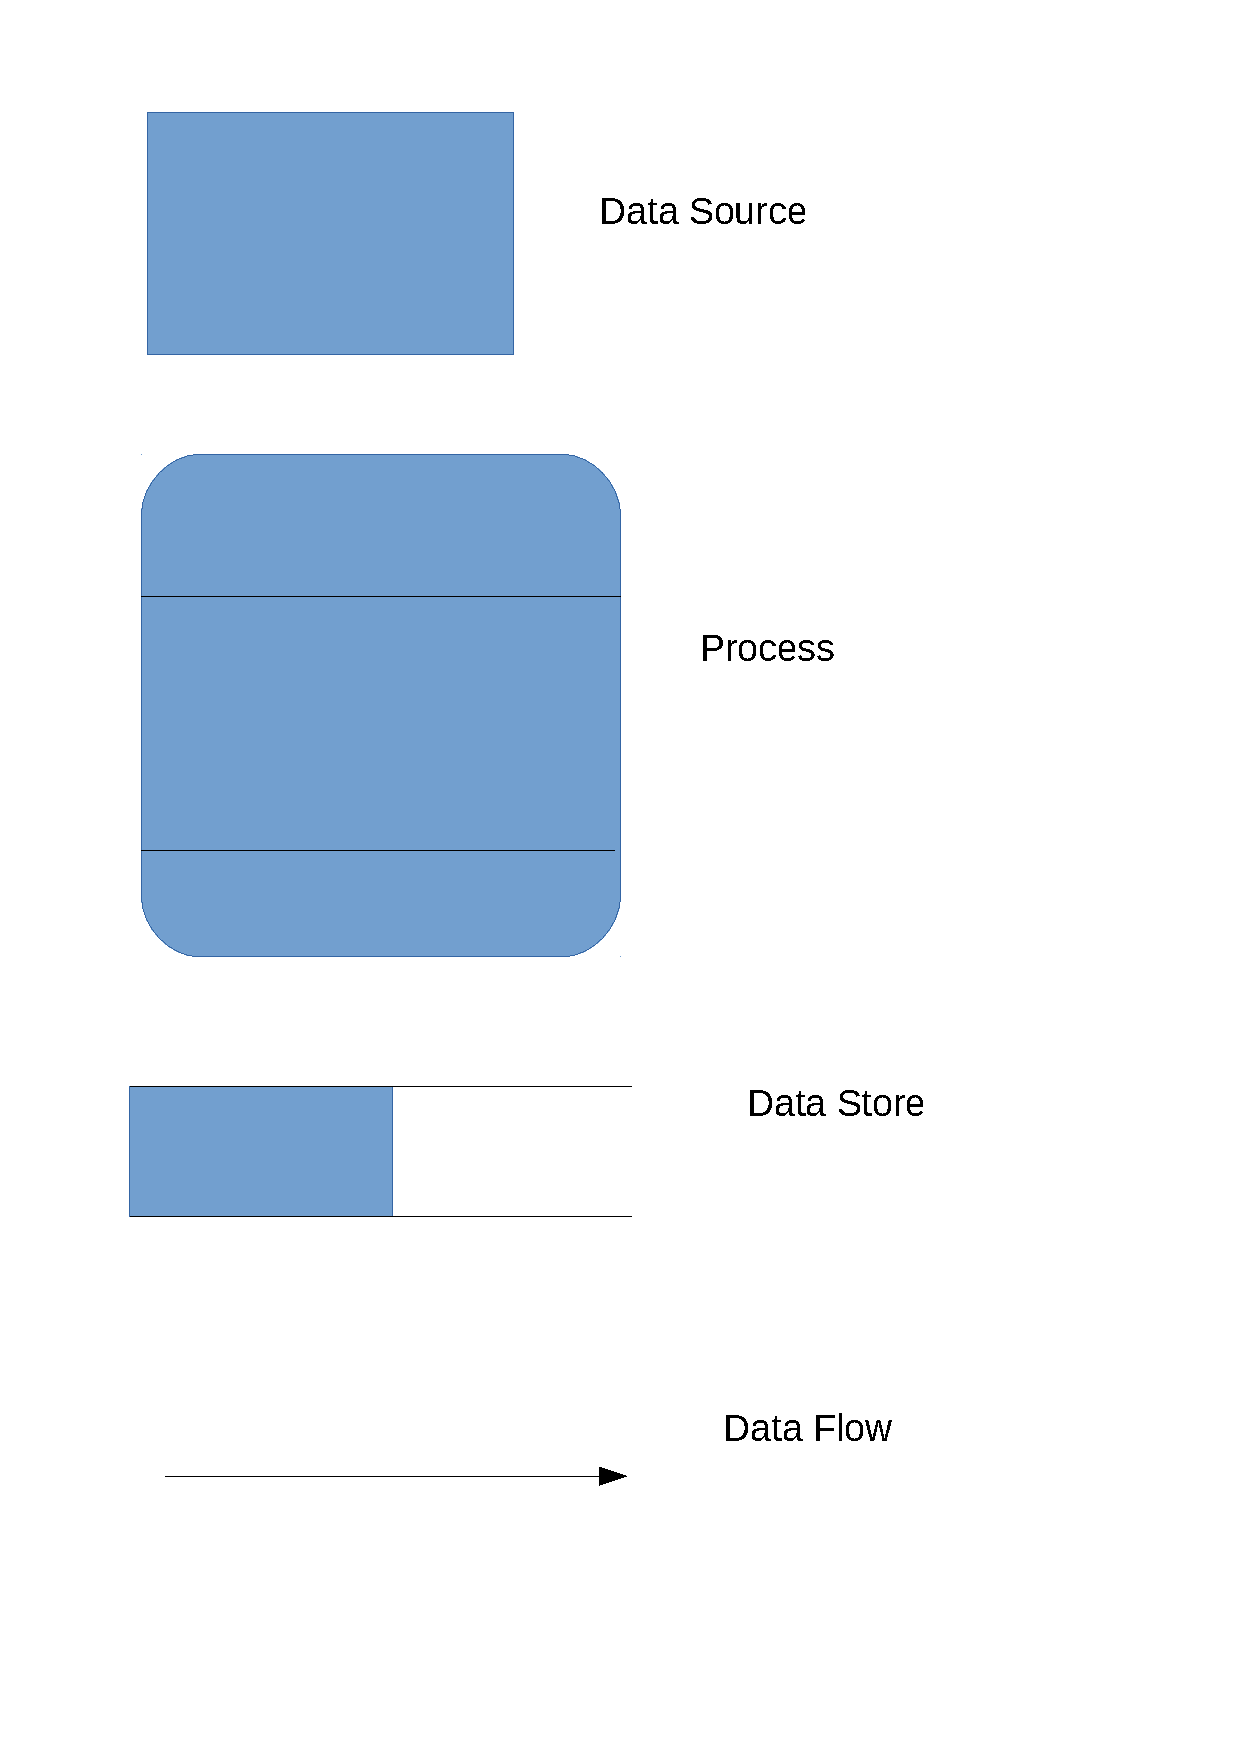
\includegraphics[width=\textwidth]{./Analysis/images/key.pdf}
    \caption{This is the key for the following data flow diagrams.} \label{fig:data_flow_diagram_key}
\end{figure}

\begin{figure}[H]
    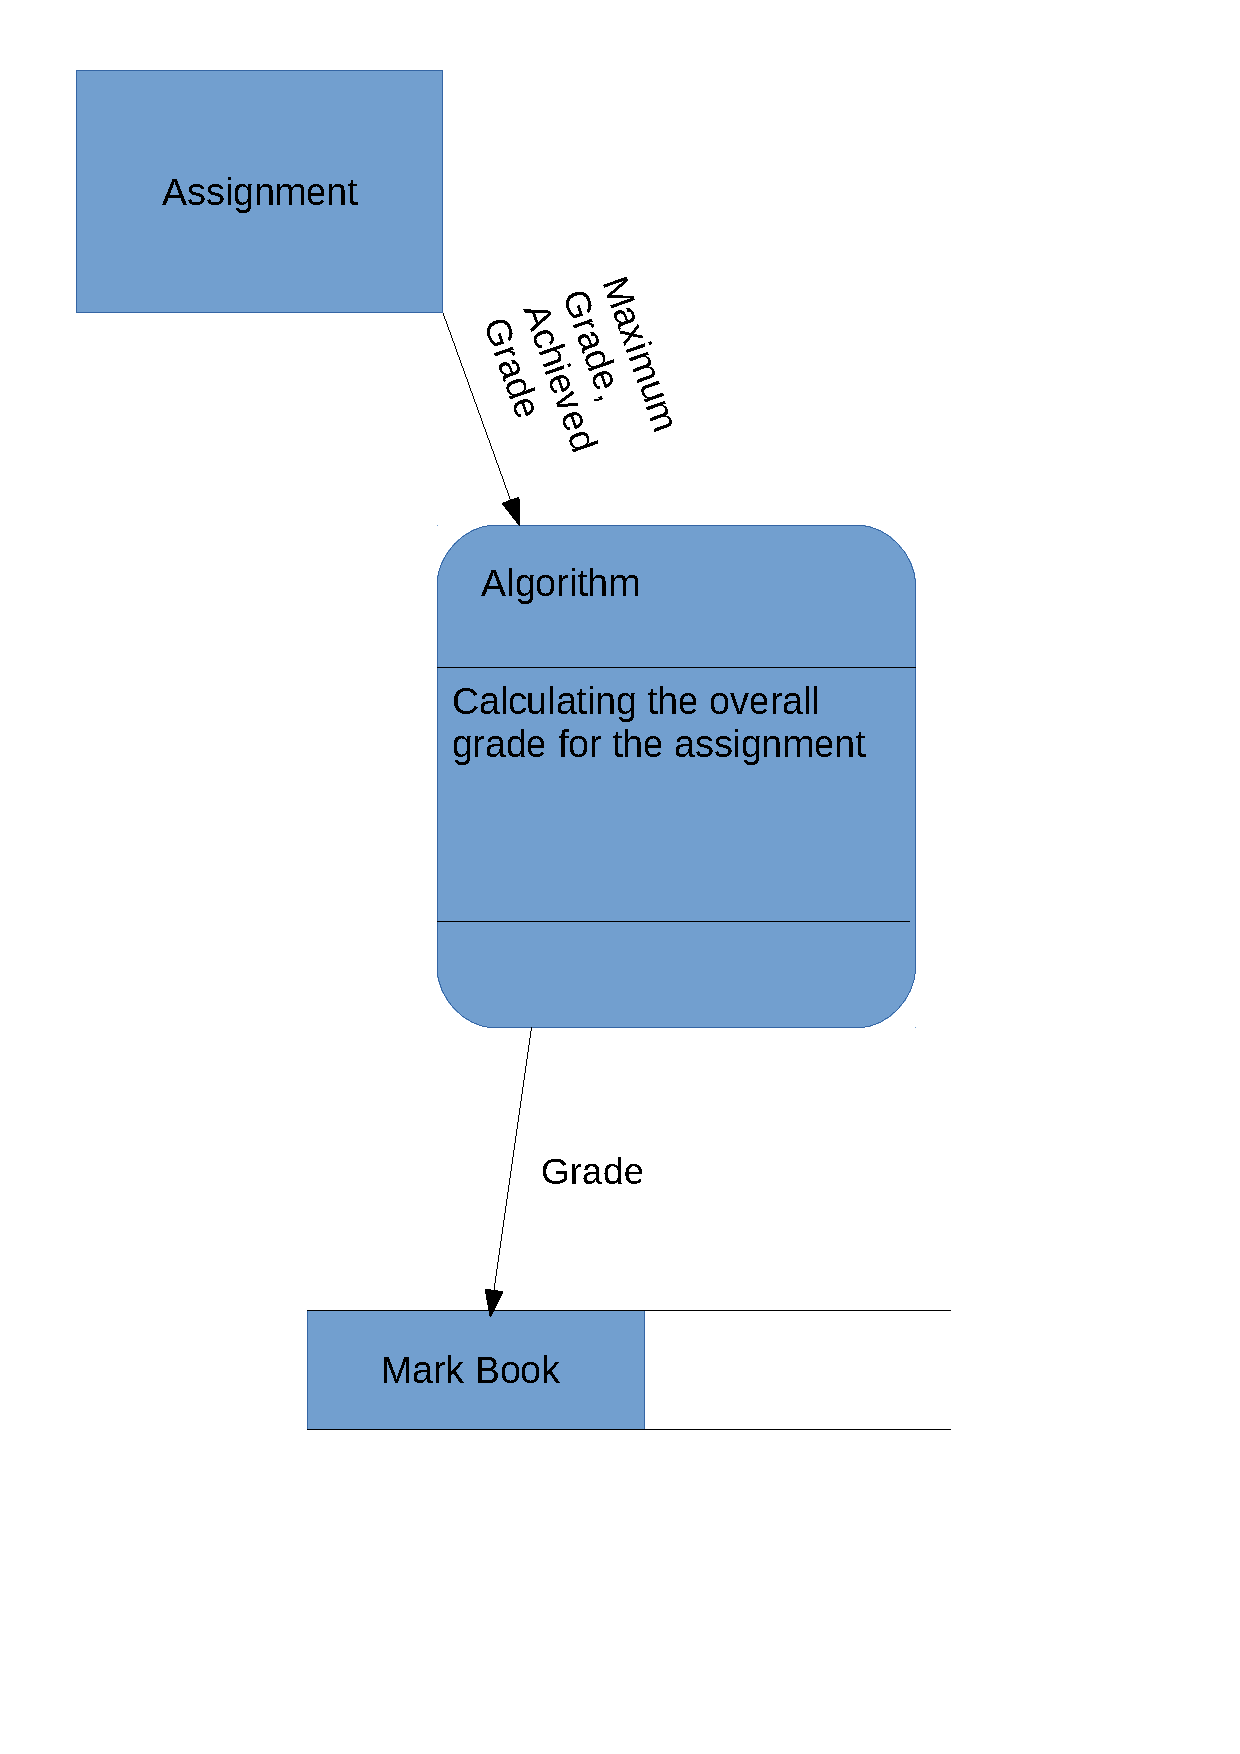
\includegraphics[width=\textwidth]{./Analysis/images/DataFlowDiagrams.pdf}
\end{figure}

\begin{figure}[H]
    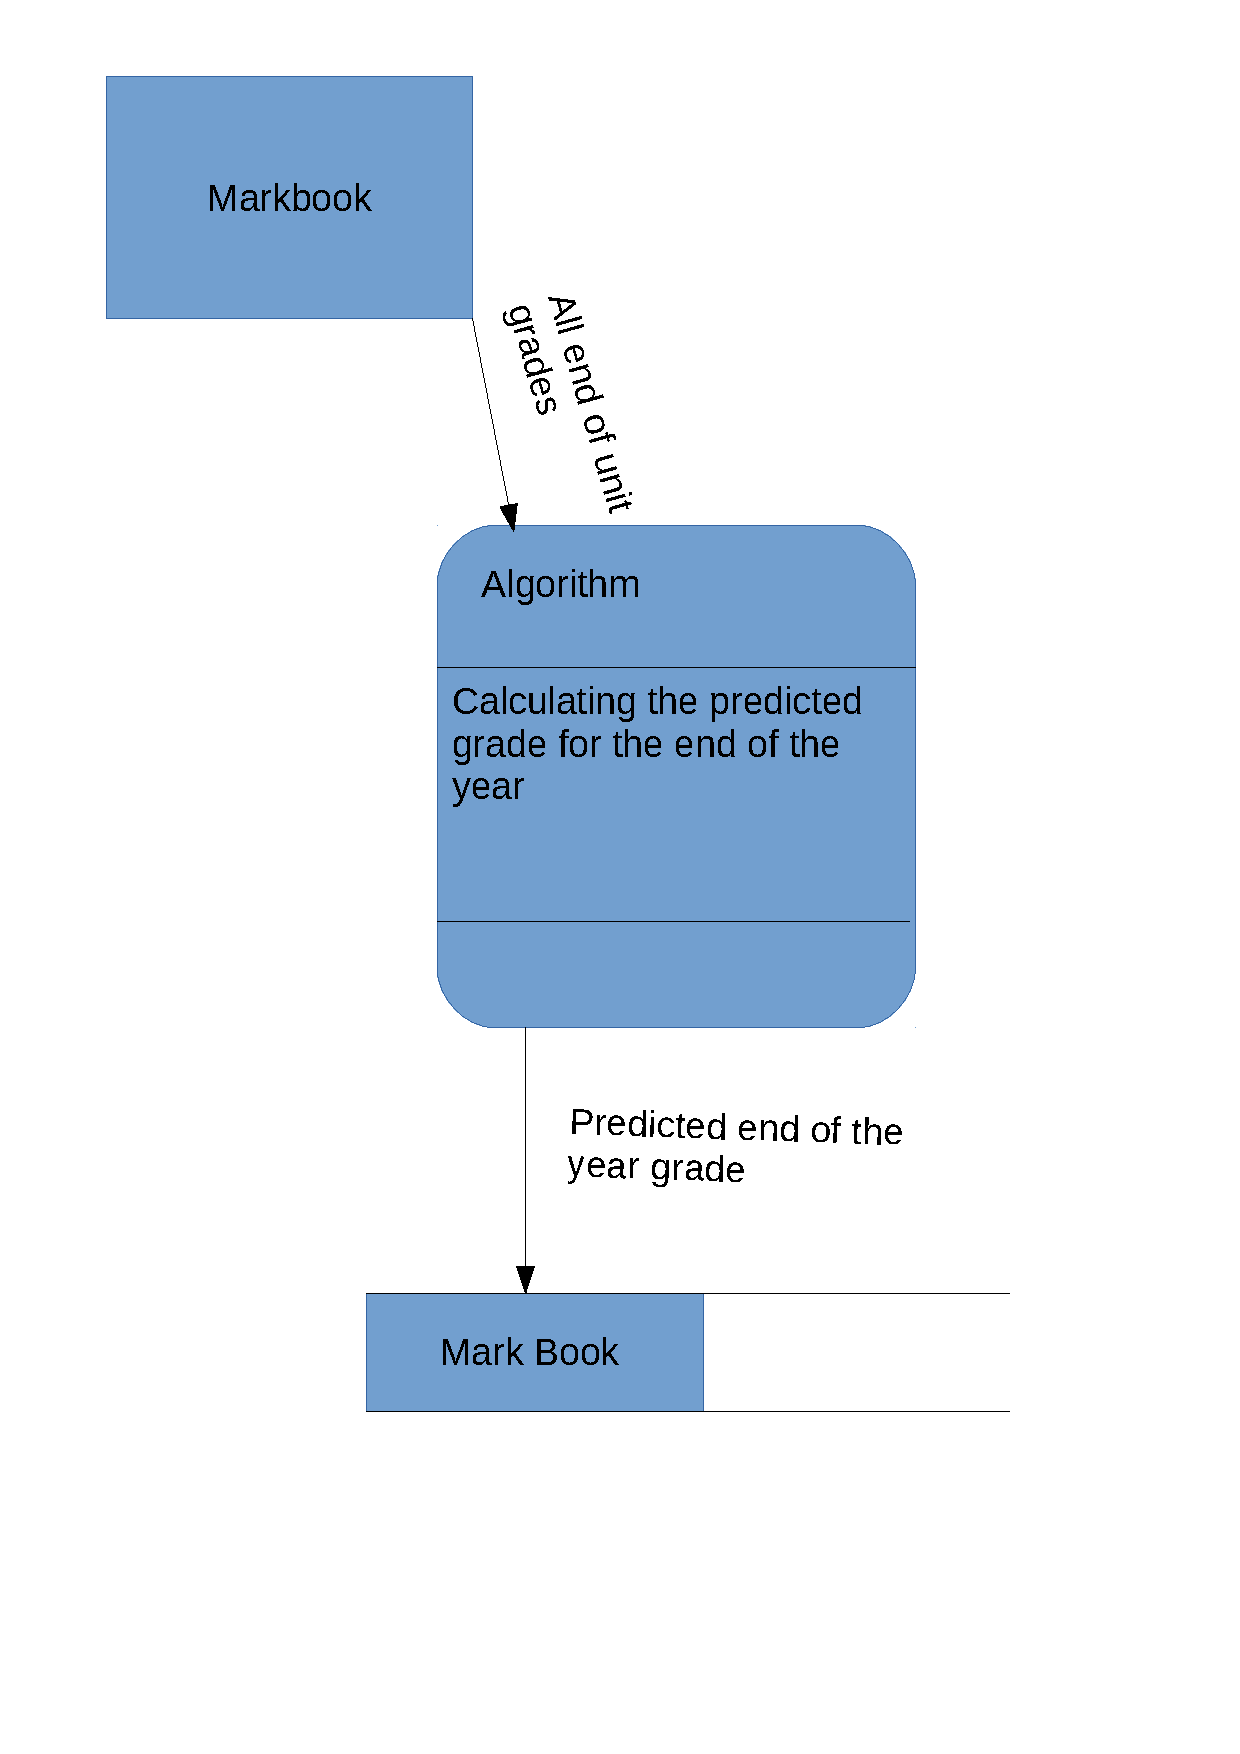
\includegraphics[width=\textwidth]{./Analysis/images/DataFlowDiagrams2.pdf}
\end{figure}

\subsubsection{Input Forms, Output Forms, Report Formats}

\subsection{The proposed system}

\subsubsection{Data sources and destinations}

\subsubsection{Data flow diagram}

\subsubsection{Data dictionary}

\subsubsection{Volumetrics}

\section{Objectives}

\subsection{General Objectives}

\subsection{Specific Objectives}

\subsection{Core Objectives}

\subsection{Other Objectives}

\section{ER Diagrams and Descriptions}

\subsection{ER Diagram}

\subsection{Entity Descriptions}

\section{Object Analysis}

\subsection{Object Listing}

\subsection{Relationship diagrams}

\subsection{Class definitions}

\section{Other Abstractions and Graphs}

\section{Constraints}

\subsection{Hardware}

\subsection{Software}

\subsection{Time}

\subsection{User Knowledge}

\subsection{Access restrictions}

\section{Limitations}

\subsection{Areas which will not be included in computerisation}
\subsection{Areas considered for future computerisation}

\section{Solutions}

\subsection{Alternative solutions}

\subsection{Justification of chosen solution}
